\section{Impact Analysis}
An impact analysis serves the purpose of helping a developer understand the implications and impact of performing a refactor or introducing a feature into a software project. This is especially relevant, as the group consists of 5 total members, each refactoring their own feature, which could very quickly result in overlapping code changes, code constantly breaking and the end product becoming unstable.

To perform this impact analysis, we're making use of the program featureous and FeatureEntryPoint annotations to annotate parts of the program that is planned to be refactored. By doing this, we can gain a further understanding of the interconnectivity of the program and see how the features overlap code-wise.

The FeatureEntryPoints created for my feature are for the following methods and constructors.

\begin{itemize}
    \item OpenFileAction constructor
    \item OpenRecentFileAction constructor
    \item actionPerformed in OpenFileAction.java
    \item openViewFromURI in OpenFileAction.java
    \item showDialog in OpenFileAction.java
    \item createDialog in OpenFileAction.java
\end{itemize}

Based on these FeatureEntryPoints, the generated report can be used to analyze the impact of the feature.

\subsection{Featureous Feature-Code Characterization}
\begin{figure}[H]
    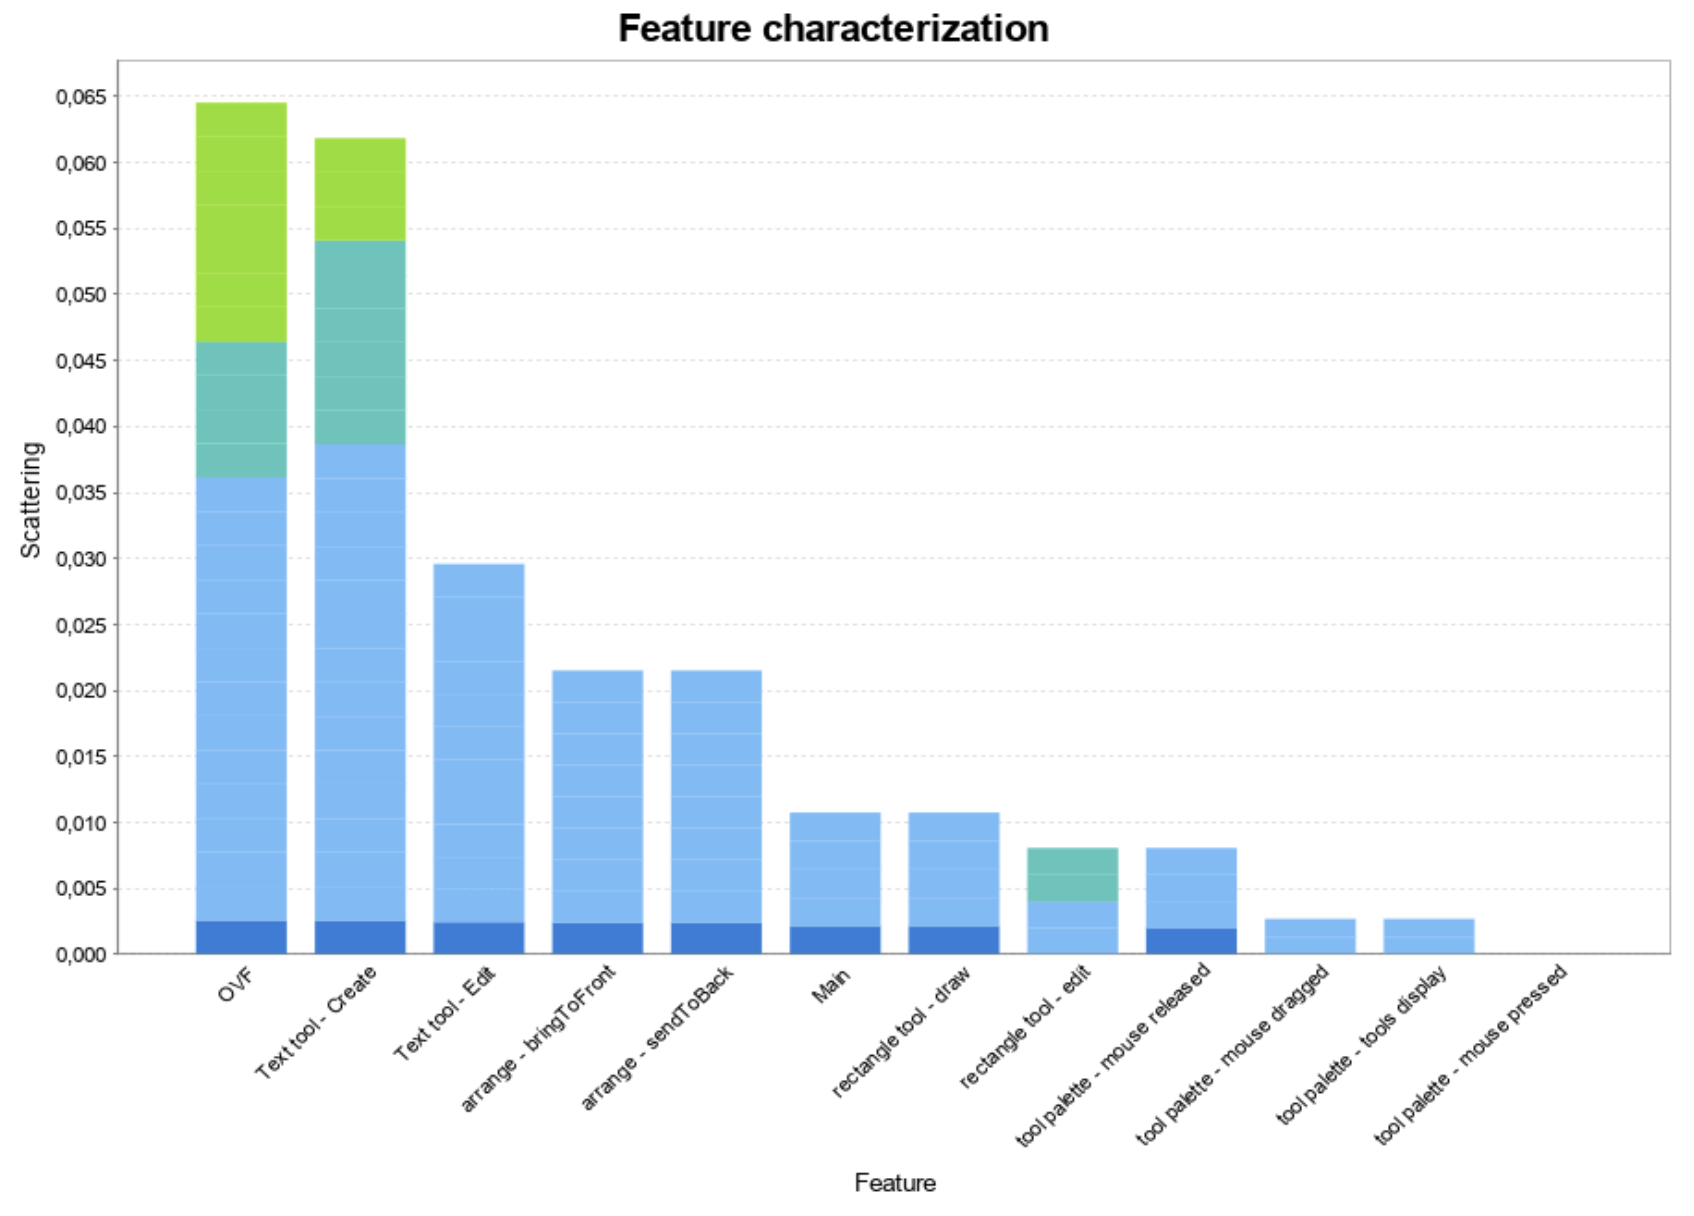
\includegraphics[width=\textwidth]{Images/featurecharacterization.png}
    \caption{Feature-Code Characterization}
\end{figure}
The above graph from featureous shows that my feature, here annotated as OVF, has a great deal of overlap with other features and is very scattered in the codebase. This means, that when refactoring, I need to be extra careful not to accidentally break other features, causing additional refactoring between me and another team member to be necessary.

\subsection{Feature Correlation Grid}
\begin{figure}[H]
    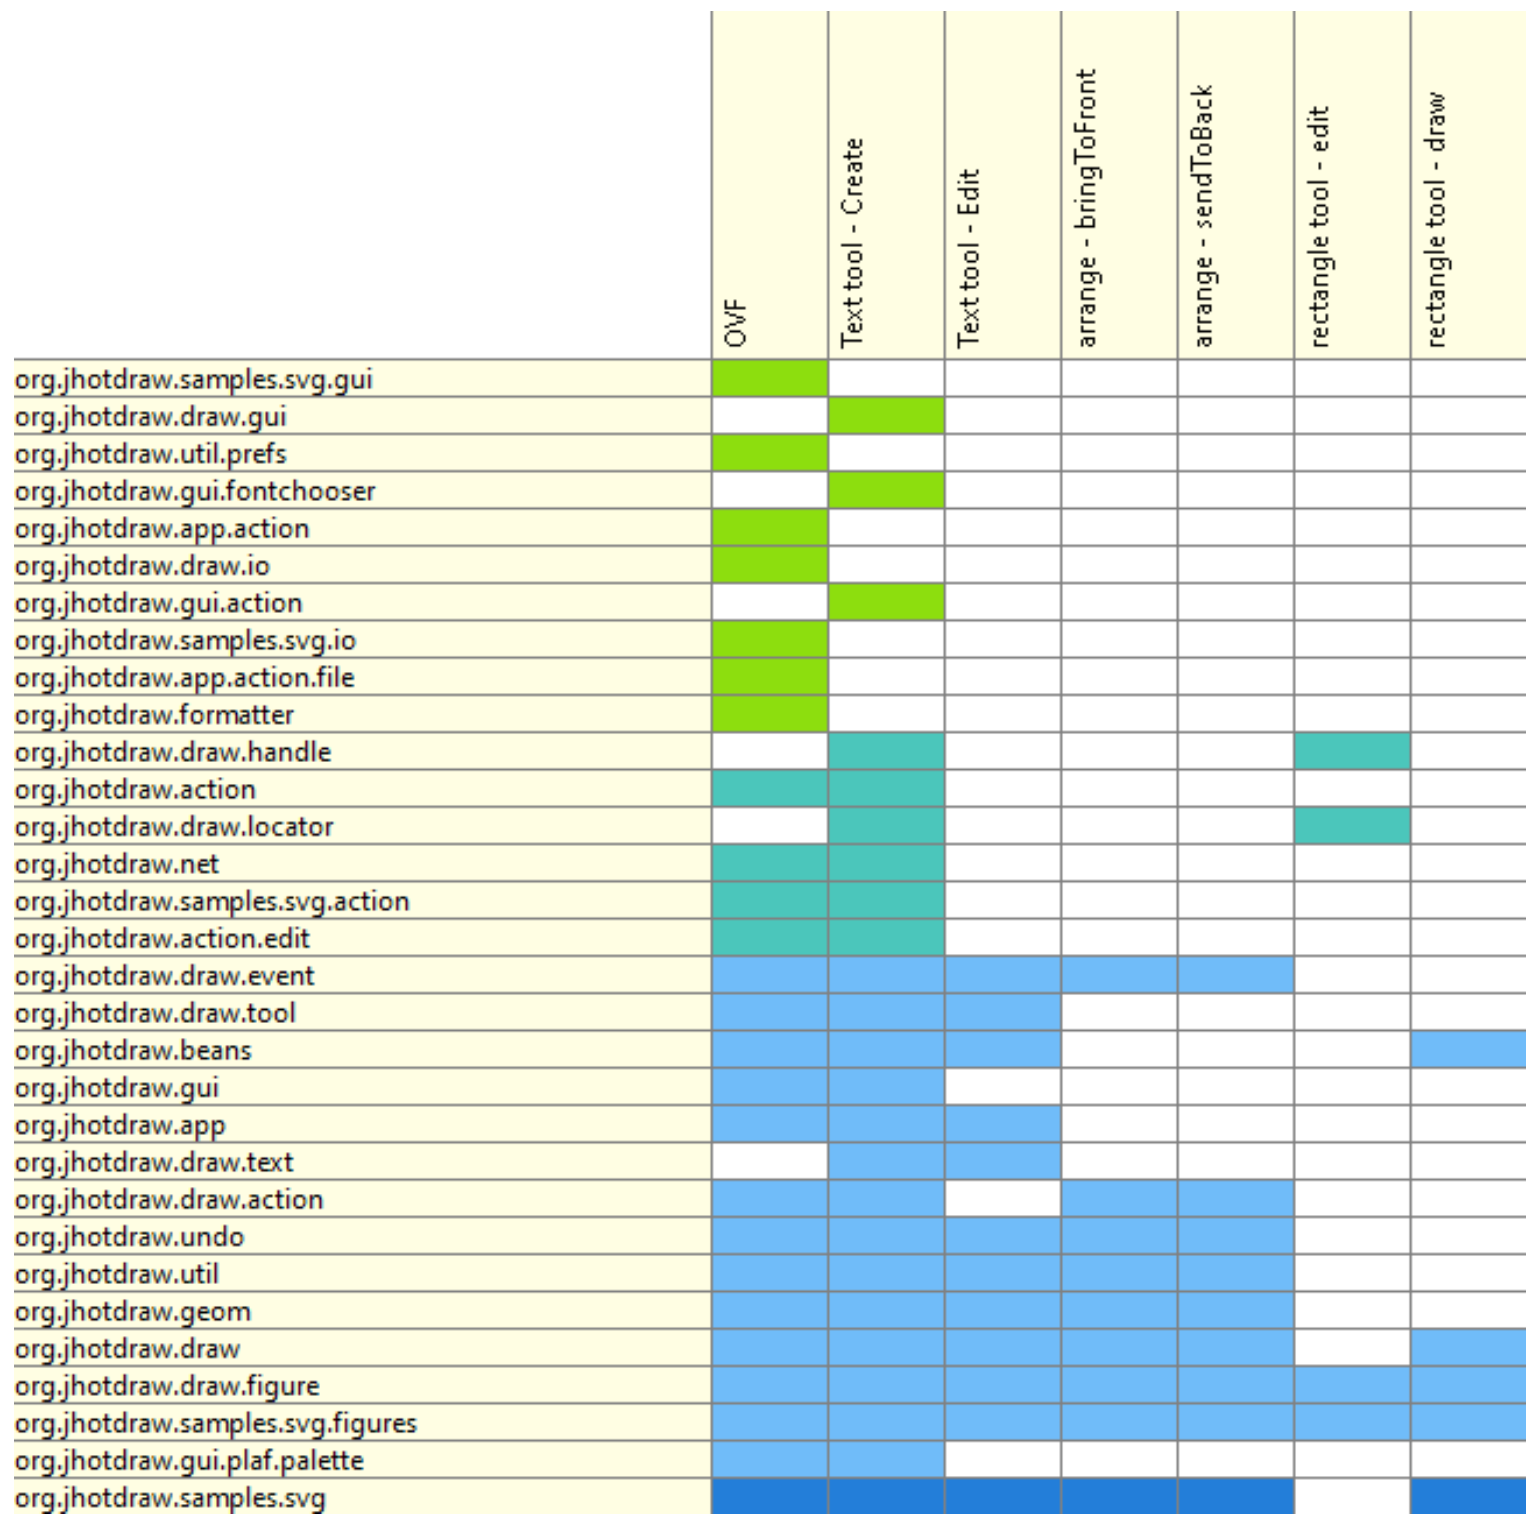
\includegraphics[width=\textwidth]{Images/featureousgrid.png}
    \caption{Feature Correlation Grid}
\end{figure}
Reading the grid reveals, that my feature has great entanglement with other features. There are several reasons why this could be the case. Firstly, my feature handles many things. Performing IO to load files, placing these image files in the GUI, drawing said feature on the screen and more. Therefore, the entanglement on display doesn't necessarily mean, that refactoring will be difficult; it does however show, that we should be wary when refactoring and extra careful that core features aren't broken when refactoring.

\subsection{Feature Correlation Graph}
\begin{figure}[H]
    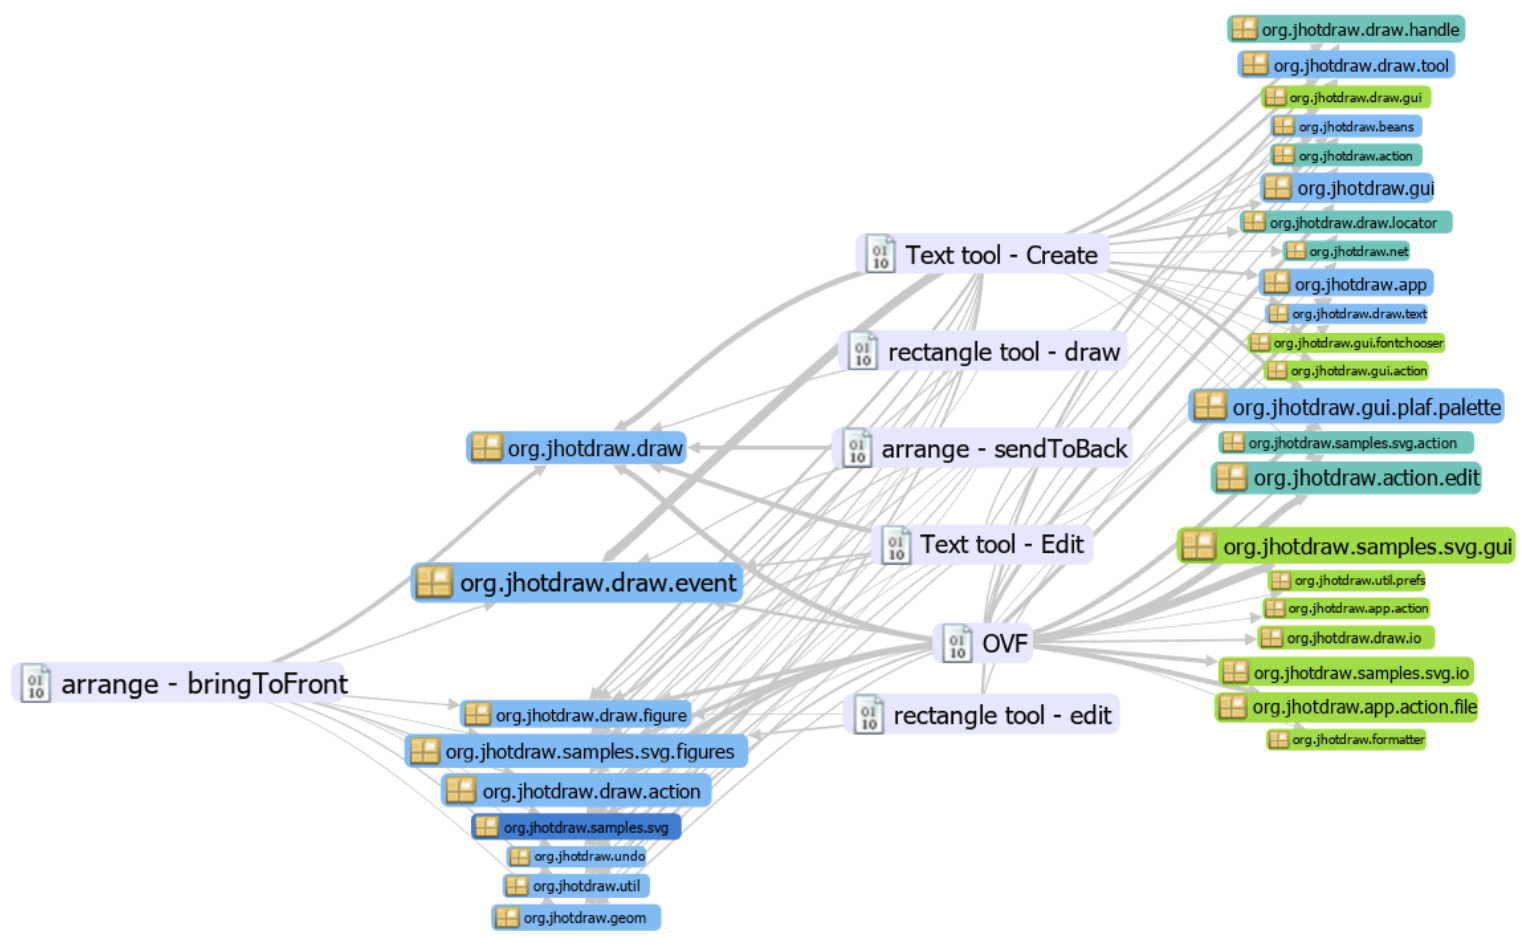
\includegraphics[width=\textwidth]{Images/featureousgraph.png}
    \caption{Feature Correlation Graph}
\end{figure}
The graph generated by the Featureous doesn't give us a lot of new information, it does however present it in another way, which gives further evidence to the fact, that while the code overlap previously seemed to be deeply ingrained, the overlaps happen in key packages such as the draw event package, figures, action etc. many of which, we won't be touching for the coming refactor or will be extra careful not to break.

\subsection{Feature Relations Characterization}
\begin{figure}[H]
    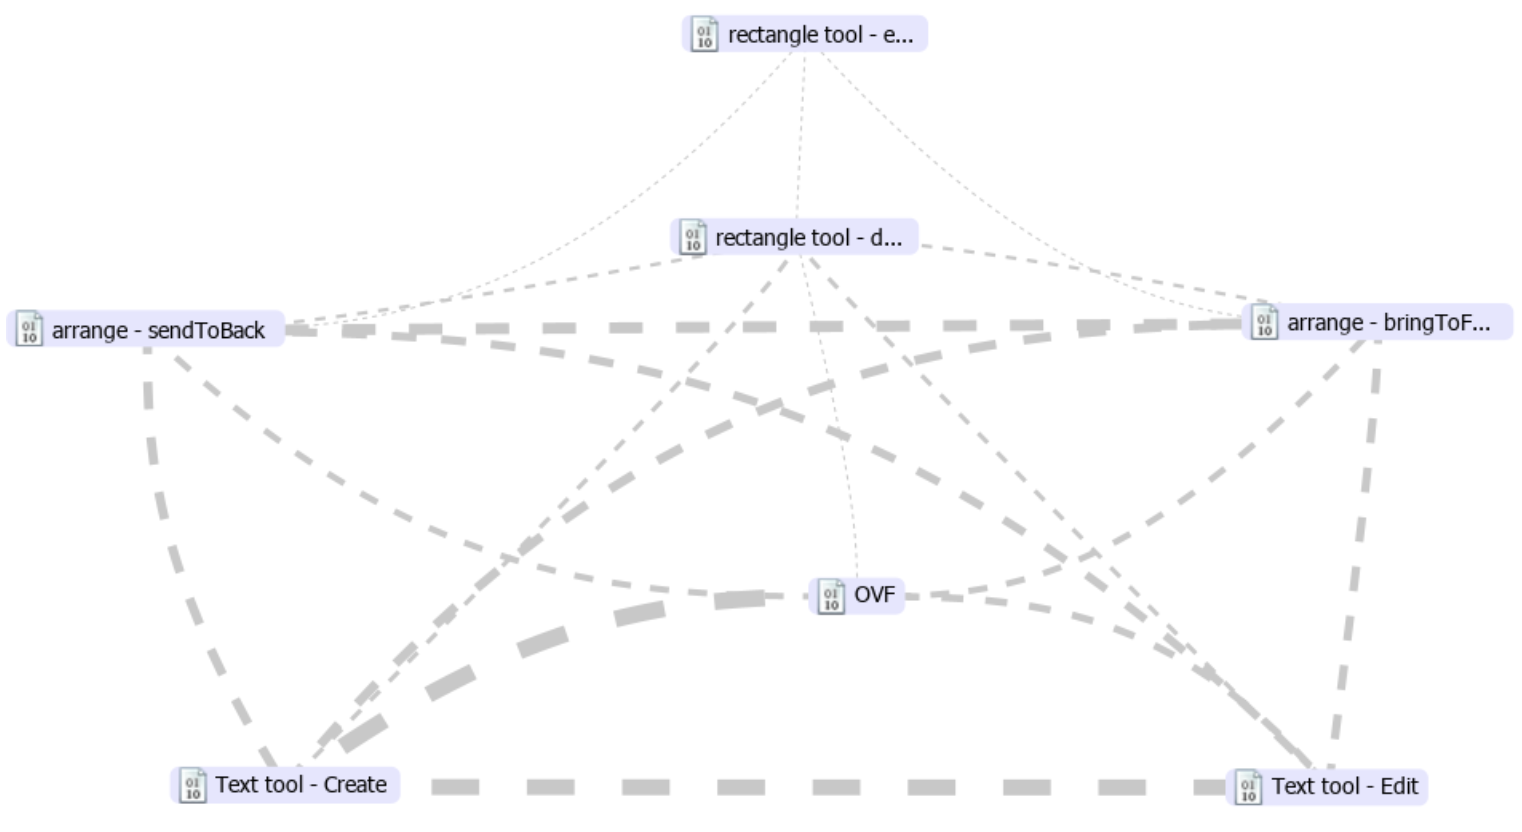
\includegraphics[width=\textwidth]{Images/featureousrelations.png}
    \caption{Feature Relations Characterization}
\end{figure}

Yet another visualization tool of the Featureous software, is the feature relations characterization, which is a simpler visualization, showing the amount of shared relations between the different features with a dashed line, increasing in thickness directly proportional to the amount of shared code. This is helpful if, like our feature correlation graph, the amount of packages on display is hard to read.

While a useful tool in many contexts, in my case, I feel it doesn't help me a lot, as my feature seemingly connects to most other features in one way or another and doesn't help me gain an entry point into analyzing my feature's impact.

\subsection{Impact Analysis}
The impact of the feature that I will be refactoring can be broken down in a table of classes and packages, helping with a general overview of the things that I need to be wary of when refactoring. These will be marked by one of the three following tags.

\begin{itemize}
    \item \textbf{Unchanged}: These are classes that I visited in my search for relevant classes, but will not be touching.
    \item \textbf{Propagating}: These are classes that I looked at, and helped me find the correct classes that I was looking for.
    \item \textbf{Changed}: These are classes that I have planned to refactor based on my analysis.
\end{itemize}

% TODO: FILL THIS OUT
\begin{longtblr}[caption = {The list of all the packages visited during impact analysis.}]{|l|l|l|l|}
    \hline
    \bf{Package name} & \bf{\# of classes} & \bf{Tool used} & \bf{Comments} \\
    \hline
    \bf{action}       & \bf{}              & \bf{}          & \bf{}         \\
    \hline
    \bf{action.file}  & \bf{}              & \bf{}          & \bf{}         \\
    \hline
    \bf{action.app}   & \bf{}              & \bf{}          & \bf{}         \\
    \hline
    \bf{}             & \bf{}              & \bf{}          & \bf{}         \\
    \hline
\end{longtblr}
